%\documentclass[10pt]{article}
%\usepackage[usenames]{color} %used for font color
%\usepackage{amssymb} %maths
%\usepackage{amsmath} %maths
%\usepackage[utf8]{inputenc} %useful to type directly diacritic characters
%\begin{document}
%%19.8.2008

\section* {Curriculum Vitae}
%\newpage
%\cleardoublepage

%\pagestyle{plain} \setlength{\topmargin}{0pt}
%\setlength{\headheight}{0pt} \setlength{\headsep}{0pt}
%\setlength{\voffset}{0pt}

%\enlargethispage{60pt}

\newcommand{\rubrique}[1]{{\textit{\textbf{\large#1}}}\smallskip\\}
\parindent=0in
\addtolength{\parskip}{1.4em}


\small

\begin{minipage}[t]{\textwidth}
    \begin{minipage}[b]{0.5\textwidth}
        \textbf{Julien COLOMB, PhD} in Biology\\
        Schillerpromenade 4\\
        12049 Berlin\\
        julien.colomb@fu-berlin.de\\
         \\
        https://github.com/jcolomb\\
         http://orcid.org/0000-0002-3127-5520\\
         \\
   
        \textbf{Birth: 9 April 1979 in Sion (CH)}\\
        \textbf{Married, two children}\\
        \textbf{Swiss}
         
    \end{minipage}\hfill
    \begin{minipage}[b]{0.5\textwidth}
        \begin{flushright}
            \fbox{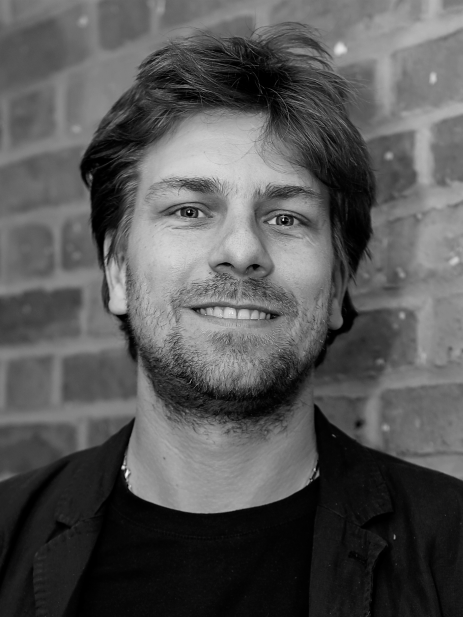
\includegraphics[scale=0.3] {Figures/photo_CV.png}}
        \end{flushright}
    \end{minipage}
\end{minipage}\\

\rubrique{Summary}
After 12 years spent on fundamental research (neuro-genetics) in which I gathered skills in experimental design, team leading and student teaching, I got most interested in open science and research reproducibility as well as the digital tools helping scientists to achieve it.
I would like to apply these novel knowledge %while doing research and mentoring students.
to bring open science principles forward.

\rubrique{Research activities}
%
\parbox{0.15\textwidth}{2017 - present}\hfill
\parbox[t]{0.83\textwidth}{Postdoctoral fellow,
       HU  (\textbf{Berlin}, Germany),
        by Prof. Y. Winter\\
        Analysing mulitdimensional dataset: the homecagescan case.}
%
\parbox{0.15\textwidth}{2015 - 2016}\hfill
\parbox[t]{0.83\textwidth}{Postdoctoral fellow,
       HU \& Charit\'e (\textbf{Berlin}, Germany),
        by Prof. Y. Winter\\
        Animal core facility director and project manager.}
 %       
\parbox{0.15\textwidth}{2014 - 2015}\hfill
\parbox[t]{0.83\textwidth}{Postdoctoral fellow,
       HU \& Charite (\textbf{Berlin}, Germany),
        by Prof. Y. Winter\\
        working on Phenobase.}
%
%
\parbox{0.15\textwidth}{2009 -2013}\hfill
\parbox[t]{0.83\textwidth}{Postdoctoral fellow,
       FU (\textbf{Berlin}, Germany),
        by Prof. B. Brembs\\
        working on "the what and where of operant learning in \textit{Drosophila}".}
   %     
                \parbox{0.15\textwidth}{2007-2008}\hfill
\parbox[t]{0.83\textwidth}{Postdoctoral fellow,
       ESPCI (\textbf{Paris}, France), by Dr. T. Preat\\
        working on "appetitive learning in \textit{Drosophila}".
        }


\rubrique{Commercial activities}
%
\parbox{0.15\textwidth}{2016-present}\hfill
\parbox[t]{0.83\textwidth}{Freelance scientist,\\
        Animal core facility (Charit\'e): organisation lead, data analysis in R,
        Phenobase (Exist, HU): literature curation.}
%        
\parbox{0.15\textwidth}{2012-present}\hfill
\parbox[t]{0.83\textwidth}{Founder and CEO 
       of Drososhare GmbH (Berlin, Germany),
        facilitating fruit fly transactions between scientists}

  
% \rubrique{Non-commercial activities}       
% \parbox{0.15\textwidth}{2015- present}\hfill
%\parbox[t]{0.83\textwidth}{Organisation of the Berlin Open Science meetup:\\
%- Discussion and brainstorming on open science themes (Reproducible Research, Open Access, peer review) \\
%- Organisation of the open con satellite}     
%
% \rubrique{Non-commercial activities}       
% \parbox{0.15\textwidth}{2015- present}\hfill
%\parbox[t]{0.83\textwidth}{Part of the march for science Berlin Orga team:\\
%we organised a protest in 2017 (11000 people) and are using this momentum to make bridges between science and society}   
                
        
\rubrique{Education}
\parbox{0.15\textwidth}{2016}\hfill
\parbox[t]{0.83\textwidth}{FELASA B. HU Berlin
        }
\parbox{0.15\textwidth}{2013}\hfill
\parbox[t]{0.83\textwidth}{Moderation \& management (Continuing Education), FU Berlin/Artop.
        }
\parbox{0.15\textwidth}{2006}\hfill
\parbox[t]{0.83\textwidth}{PhD in Biology,
        University of Fribourg (\textbf{Fribourg}, Switzerland).\\
        PhD dissertation: ``The chemosensory system of \textit{Drosophila} larvae: neuroanatomy and behaviour''
        Thesis director: Prof. R.F Stocker}
\parbox{0.15\textwidth}{2002}\hfill
\parbox[t]{0.83\textwidth}{Diploma in Biology,
        University of Fribourg (\textbf{Fribourg}, Switzerland)
        %\\
        %Subject: "Anatomical and functional studies of the chemosensory system of the \textit{Drosophila} larva suggest the presence of a gustatory target area in the antennal lobe?"
        }
\parbox{0.15\textwidth}{1998}\hfill
\parbox[t]{0.83\textwidth}{``Maturit\'e f\'ed\'erale type C'' (scientific subsection),
in the "Coll\`ege de la royale Abbaye de St. Maurice"}

\rubrique{Languages} French (mother tongue), English (fluent),
German (fluent), Spanish (basics).

\rubrique{Research output}
%
%
 8 research papers (7 first author), 3 reviews, 1 Scienceopen collection, 3 Open source software (2 main author), Meeting Presentations > 25\\
 https://orcid.org/0000-0002-3127-5520\\
 https://github.com/jcolomb\\
 %RG score = 17.06 (>60\%),



%\rubrique{Overview} 
%The three papers published indicate the relative abundance and quality at the research undergone during my PhD. On the other hand, teaching experience and meeting organization, as well as involvement in the theatre group of the university, show my interest in academic life.
%\newpage

\rubrique{Supervision of student}
\parbox{0.15\textwidth}{2010-2014}\hfill
	\parbox[t]{0.83\textwidth}{Co-supervisor of the PhD student Christine Damrau
(with Dr. B.Brembs) on the role of octopamine in reward, motivation and motor control in  \textit{Drosophila}.}
\parbox{0.15\textwidth}{2008}\hfill
	\parbox[t]{0.83\textwidth}{Co-supervisor of the PhD student S\'everine Trannoy
(with Dr. G. Isabel and Dr. N. Gervasi) on the role of dopamine in appetitive learning consolidation in  \textit{Drosophila}.}
\parbox{0.15\textwidth}{2005}\hfill
\parbox[t]{0.83\textwidth}{Co-supervisor of the diploma work of Claire Huguenin
(with Dr. A. Ramaekers) on the role of NO in olfactory discrimination in \textit{Drosophila} larvae.}





\rubrique{Teaching experience}
\parbox{0.15\textwidth}{2016}\hfill
\parbox[t]{0.83\textwidth}{Animal models of neuropathy, (master student, 2x2h lecture, organisation)}

\parbox{0.15\textwidth}{2012}\hfill
\parbox[t]{0.83\textwidth}{Genetik (bachelor student, 2 x 3 h. lecture, 2x 1h. seminar)}
\parbox{0.15\textwidth}{2012}\hfill
\parbox[t]{0.83\textwidth}{Neurogenetik. (master student, 2 x 2 h. lecture, 2x 1h. seminar)}
\parbox{0.15\textwidth}{2011}\hfill
\parbox[t]{0.83\textwidth}{Practical course neurobiology. (7 x 4 h., Practical course supervision)}
\parbox{0.15\textwidth}{2011}\hfill
\parbox[t]{0.83\textwidth}{Entwicklung der Insekten [Insect development] (2 h. lecture)}
 
\parbox{0.15\textwidth}{2006}\hfill
\parbox[t]{0.83\textwidth}{Fluorescence and Confocal Microscopy (master student, 3h. lecture)}
\parbox{0.15\textwidth}{2003-2006}\hfill
\parbox[t]{0.83\textwidth}{Studying behavior. (master student, 2 h. lecture)}
\parbox{0.15\textwidth}{2003-2005}\hfill
\parbox[t]{0.83\textwidth}{Developmental- and Neurogenetics %An introduction to learning and memory and their molecular mechanisms.
(master student, 2 h. lecture%, part of the lecture course "Developmental- and Neurogenetics" given by R.F. Stocker
).}


%
%\rubrique{Approved grants}
%\parbox{0.15\textwidth}{2010}\hfill
%  \parbox[t]{0.83\textwidth}{DFG
%  Forschungsgruppe "biogenic amines in insects",
%  cowritten with Dr. Brembs.}
%\parbox{0.15\textwidth}{2009}\hfill
%  \parbox[t]{0.83\textwidth}{SNF for avanced researchers: PA00P3-124141 - "The what and where of operant learning in \textit{Drosophila}" }
%\parbox{0.15\textwidth}{2007}\hfill
%\parbox[t]{0.83\textwidth}{SNF for prospective researchers: PBFR33-116951 - "Memory phases of reward learning in \textit{Drosophila melanogaster}"}%\vskip 0.1em
%
%
%
%%\newpage
%\rubrique{Organization of conferences}
%\parbox{0.15\textwidth}{2004}\hfill
%\parbox[t]{0.83\textwidth}{Co-organizer of a PhD meeting, in Cerniat. (30 participants)}\vskip 0.1em
%
%
%%\rubrique{Summer jobs}
%%\parbox{0.15\textwidth}{1996--2001}\hfill
%%\parbox[t]{0.83\textwidth}{Summer job in the company of building and civil engineering CONFORTI SA.}\vskip 0.1em
%
%
%
%
%
%
%
%\rubrique{Reviewer for the following journals}
%PRE-PUBLICATION: Current Biology, Proceedings of the royal society B,  The Journal of Experimental Biology, learning and memory, PLoS one, JEAB
%\\POST-PUBLICATION: Associate member of faculty of 1000 
%
\rubrique{Computer skills}
\emph{Organisation}: Outlook, Access, labfolder;
\emph{Publishing}: \LaTeX, Office, overleaf, markdown, html, figshare;
\emph{Image processing}: Photoshop, Illustrator, Image J; 
\emph{Programming and data analysis}:  R, Rmarkdown, shiny, Git, Labview;
\emph{Collaborative working}:  Github, redmine

\rubrique{Other tasks}
%Founding of the \textit{Drososhare} startup
%\\
Organisation of the Berlin Open Science meetup:\\
Part of the march for science Berlin Orga team:\\
Creation of the T. Preat's and R.F. Stocker's lab website.
\\
Co-director in the theater group "les apostrophes" in
2006

%\\Cashier of and actor in the theater group "les apostrophes" in 2002-2005.

%\subsection* {Project management and leadership skills}
%
%During my PhD thesis and my post-doctoral experience, I both developed and demonstrated the abilities of independent initiative and creative thinking. I had the opportunity to propose, develop and then bring to fruition my own projects. I also presented my work in different congresses; in particular, I gave an oral presentation in the 2006 neurofly meeting, which gathered the whole community of neuroscientists working on \textit{Drosophila}.
%I already took great part in the redaction of the papers of my thesis, a skill that I developed further.
% Furthermore, I have been learning to elaborate long term and more integrated projects, thanks to my post-doctoral training.
%%In addition, I recently modified a test measuring feeding behaviors for the motivation test described in section~\ref{sec:paradigms}.
%All these elements demonstrate my abilities to take initiative and to manage a project from its beginning to its end. 
%I also took part in the supervision of students. Moreover, as a co-director in the theatre group of the University during my thesis, I also gained experience in the difficult task of group management. 

\newpage

%
\subsection*{RESEARCH PRODUCTS}



\rubrique{Open source Software}
\begin{itemize}
\begin{sloppypar}
%
\item(2011-2013) CeTrAn 1.4 to 4.0, 
developed on Github (https://github.com/jcolomb/CeTrAn).
Used for more than three research papers.

\item(2016-2017) Viewer data concatenator and flystockcleaner (shiny apps).

\item(2013-2017) Collaborating on osfR, Rfigshare and Rflybase (on github).

%
%
\end{sloppypar}
\end{itemize}

\rubrique{Peer review publications}
%5 1st author research paper,
%2 review (from which 1 book chapter),
%1 extra-view article\\
%"`publish or perish"` statistics
%Papers:	6	Cites/paper:	3.67	h-index:	3	
\subsubsection{Five most important publications:}
\label{sec:FiveMostImportantPublications}

\begin{sloppypar}
%\newcommand{\enquote}[1]{``#1''}
\providecommand{\bibinfo}[2]{#2}
%
%In prep.
%
 %

\begin{itemize}   
 
\item  (\bibinfo{year}{2016}).
  \bibinfo{author}{\textbf{Julien~Colomb}} and \bibinfo{author}{Bj\"{o}rn~Brembs}. \\
\newblock \enquote{\bibinfo{title}{ PKC in motorneurons underlies self-learning, a form of motor learning in Drosophila}}
\newblock \bibinfo{journal}{PeerJ}
  (\bibinfo{pages}{e1971}).
  \\cited 3 times%, from which 0 reviews and 1 self 




 
\item  (\bibinfo{year}{2014}).
  \bibinfo{author}{\textbf{Julien~Colomb}} and \bibinfo{author}{Bj\"{o}rn~Brembs}. \\
\newblock \enquote{\bibinfo{title}{Sub-strains of Drosophila Canton-S differ markedly in their locomotor behavior}}.
\newblock \bibinfo{journal}{F1000RESEARCH}
  (\bibinfo{pages}{3:176}).
  \\cited 15 times%, from which 0 reviews and 1 self 
  

\item   (\bibinfo{year}{2009}).  
 \bibinfo{author}{\textbf{Julien~Colomb}}, \bibinfo{author}{Laure~Kaiser}, \bibinfo{author}{Marie-Ange~Chabaud}, \bibinfo{author}{Thomas~Preat}.
\\
\newblock \enquote{\bibinfo{title}{Parametric and genetic analysis of Drosophila appetitive long-term memory and sugar motivation}}
\newblock \bibinfo{journal}{Genes Brain and Behaviour}
  (\bibinfo{pages}{8 (4): 407-415}).
   \\cited 52 times%, from which 0 reviews and 1 self
   

   

 
 
  \item  (\bibinfo{year}{2007}).
\bibinfo{author}{\textbf{Julien~Colomb}}, \bibinfo{author}{Nicola~Grillenzoni}, \bibinfo{author}{Ariane~Ramaekers}, and
  \bibinfo{author}{Reinhard F.~Stocker}.\\
\newblock \enquote{\bibinfo{title}{Architecture of the primary taste center of \textit{Drosophila melanogaster} larvae}}.
\newblock \bibinfo{journal}{J. comp. neurol.}
  (\bibinfo{pages}{502: 834-847}).
   \\  cited 72 times%, from which 2 reviews and 7 self
 %\google scholar + 2 self reviews



\item  (\bibinfo{year}{2007}).
  \bibinfo{author}{\textbf{Julien~Colomb}}, \bibinfo{author}{Nicola~Grillenzoni},
  \bibinfo{author}{Reinhard F.~Stocker}, and \bibinfo{author}{Ariane~Ramaekers}. \\
\newblock \enquote{\bibinfo{title}{Complex behavioural changes after odour exposure in \textit{Drosophila} larva}}.
\newblock \bibinfo{journal}{Anim. Behav.}
  (\bibinfo{pages}{73 (4): 579-85}).
   \\ cited 13 times%, from which 3 reviews and 2 self
   %\google scholar -1 double +1 self review
 \end{itemize}
 
\subsubsection{Other Publications }
\label{sec:OtherPublications}
\begin{itemize}


\item  (\bibinfo{year}{In revision}).
  \bibinfo{author}{ \bibinfo{author}{Christine~Damrau},  \bibinfo{author}{Naoko~Toshima}, \bibinfo{author}{Teiichi~Tanimura},  \bibinfo{author}{Bj\"{o}rn~Brembs} \textbf{Julien~Colomb}}. \\
\newblock \enquote{\bibinfo{title}{Octopamine and Tyramine contribute separately to the
counter-regulatory response to sugar deficit in Drosophila.}}
\newblock \bibinfo{journal}{Frontiers}
 \\
 


\item  (\bibinfo{year}{2014}).
  \bibinfo{author}{Ezequiel~Mendoza}, 
  \bibinfo{author}{\textbf{Julien~Colomb}},
  \bibinfo{author}{J\"{u}rgen~Rybak},
  \bibinfo{author}{Hans-Joachim~Pfl\"{u}ger}, 
  \bibinfo{author}{Troy~Zars},
  \bibinfo{author}{Constance~Scharff},
  and \bibinfo{author}{Bj\"{o}rn~Brembs}. \\
\newblock \enquote{\bibinfo{title}{\textit{Drosophila} FoxP mutants are deficient in operant self-learning}}.
\newblock \bibinfo{journal}{Plos One}
  (\bibinfo{pages}{9(6): e100648}).
  %\\cited 15 times%, from which 0 reviews and 1 self 
  

\item  (\bibinfo{year}{2012}).
  \bibinfo{author}{\textbf{Julien~Colomb}}, \bibinfo{author}{Lutz~Reiter},
  \bibinfo{author}{Jedrzej~Blaszkiewicz}, 
  \bibinfo{author}{Jan~Wessnitzer} and \bibinfo{author}{Bj\"{o}rn~Brembs}. \\
\newblock \enquote{\bibinfo{title}{Open Source Tracking and Analysis of Adult \textit{Drosophila} Locomotion in Buridan's Paradigm with and without Visual Targets.}}.
\newblock \bibinfo{journal}{Plos One}
  (\bibinfo{pages}{7(8): e42247}).
 % \\cited 34 times%, from which 0 reviews and 1 self 
  
  

\item   (\bibinfo{year}{2010}).  
 \bibinfo{author}{\textbf{Julien~Colomb}}, \bibinfo{author}{Bj\"{o}rn~Brembs} \\
\newblock \enquote{\bibinfo{title}{biology of psychology: "simple conditioning"}}
\newblock \bibinfo{journal}{Communicative and Integrative Biology}
  (\bibinfo{pages}{3 (2): 142-145}).
 %  \\cited 20 times%, from which 0 reviews and 1 self
   %
   %
   
 \item   (\bibinfo{year}{2008}).  
 \bibinfo{author}{\textbf{Julien~Colomb}}\\
\newblock \enquote{\bibinfo{title}{Discriminative learning, learning generalization and masking tests as three strategies to assess olfactory discrimination.}}
\newblock \bibinfo{book}{Animal Behaviour: New Research}
\bibinfo{pages}{185-192}
%\\ cited 0 times%, from which 0 reviews and 0 self

    \item  (\bibinfo{year}{2007}).
 \bibinfo{author}{\textbf{Julien~Colomb}*}, \bibinfo{author}{R\"{u}diger Bader*}, \bibinfo{author}{Bettina Pankratz},
\bibinfo{author}{Anne Schr\"{o}ck}, \bibinfo{author}{Reinhard F. Stocker}, and \bibinfo{author}{Michael J. Pankratz}.
\\
\newblock \enquote{\bibinfo{title}{Genetic dissection of a neural circuit underlying feeding behavior
in \textit{Drosophila}: distinct morphology of single \textit{hugin} expressing
neurons}}.
\newblock \bibinfo{journal}{J. comp. neurol.}
  (\bibinfo{pages}{502: 848-856}).\\
 * {\footnotesize the two authors participated equally to this work.}
% \\ cited 67 times%, from which at least 4 reviews and 8 self
%\google scholar

 \item   (\bibinfo{year}{2007}).  
 \bibinfo{author}{\textbf{Julien~Colomb}}, \bibinfo{author}{Reinhard F.~Stocker}\\
\newblock \enquote{\bibinfo{title}{Combined rather than separate pathway for hedonic and sensory aspects of taste in  \textit{Drosophila} larvae.}}
\newblock \bibinfo{journal}{FLY}
  (\bibinfo{pages}{1 (4): 232-234}).
% \\ cited 5 times%, from which 1 reviews and 0 self

\end{itemize}

\end{sloppypar}


%\newpage
\rubrique{Meeting presentations (4 most representative)}

\begin{itemize}
\begin{sloppypar}

\item[2016] Faster and more reproducible science: Open Science. ORAL PRESENTATION at the neurofly meeting, Creta, Greece.

%\item[2013] Genetic dissection of octopamine action in reward-related behavior and motor control in Drosophila (last author) POSTER at the SFN meeting, San Diego, USA

%
%\item[2012] PKC and dFoxP necessity for operant self-learning. 
%\\POSTER PRESENTATION at the neurofly meeting, Padova, Italy.

%\parbox{0.15\textwidth}{2005}\hfill
%\parbox[t]{0.83\textwidth}{NEUROARCHITECTURE OF THE LARVAL GUSTATORY SYSTEM.
%Poster at the CSH neurobiology of Drosophila meeting, USA,(NY)}\vskip 0.1em

%\parbox{0.15\textwidth}{2005}\hfill
%\parbox[t]{0.83\textwidth}{Les projections des neurones gustatifs: s�gr�gation selon l'organe d'origine.
%Talk at the "rencontre du club de neurobiologie des invert�br�s", Paris.}\vskip 0.1em

%\parbox{0.15\textwidth}{2004}\hfill
%\parbox[t]{0.83\textwidth}{Different sensory projections define subregions in the first gustatory
%center of Drosophila larval brain. Poster at the neurofly meeting
%in Neuch�tel}\vskip 0.1em
%
%\parbox{0.15\textwidth}{2004}\hfill
%\parbox[t]{0.83\textwidth}{Neuroanatomical studies in Drosophila melanogaster: the gustatory system.
%Talk at the PhD meeting in Cerniat, Switzerland.}\vskip 0.1em
%
%\parbox{0.15\textwidth}{2004}\hfill
%\parbox[t]{0.83\textwidth}{Food-independent learning after olfactory exposure in agar plate in Drosophila
%melanogaster larvae. Poster at the PhD meeting in Cerniat.}\vskip 0.1em
%
%\parbox{0.15\textwidth}{2004}\hfill
%\parbox[t]{0.83\textwidth}{Learning by odor exposure in agar plate. Talk at the BEHAVIOURAL NEUROBIOLOGY
%OF DROSOPHILA LARVAE meeting in W�rzburg, Germany.}\vskip 0.1em
%
%\parbox{0.15\textwidth}{2002}\hfill
%\parbox[t]{0.83\textwidth}{Functional studies of the chemosensory system of the Drosophila larva  using a new
%tool: the GAL4 / UAS-shits system. Poster at the neurofly in Dijon, France.}\vskip 0.1em
%
%\parbox{0.15\textwidth}{2002}\hfill
%\parbox[t]{0.83\textwidth}{Functional studies of the chemosensory system of the Drosophila larva  using a new tool:
%the GAL4 / UAS-shits system. Talk at the Swiss Drosophila meeting in Basel.}\vskip 0.1em
%\newpage

%\textbf{Main meetings presentation}
%
%
%

%
%\begin{sloppypar}
%\item[2012] PKC and DFoxP are necessary for operant self-learning. 
%\\POSTER PRESENTATION at the FENS meeting, Barcelona, Spain.
%
%
%\item[2011] Hide if you can't fly !?
%\\POSTER PRESENTATION at the GNS meeting, G\"{o}ttingen, Germany.

%\item[2010] The what and where of opernant learning in \textit{Drosophila}.
%\\POSTER PRESENTATION at the SNF meeting, San Diego, USA.
%%
\item[2008] New insight into appetitive Long term memory in \textit{Drosophila}.
POSTER PRESENTATION at the FENS Forum, Geneva, Switzerland.

%\item[2007] Long term memory after appetitive learning in \textit{Drosophila}.
%\\ORAL PRESENTATION at the "rencontre du club de
%neurobiologie des invert�br�s", Versailles.

\item[2006] Sub-regions in the primary taste center of \textit{Drosophila} larvae.
ORAL PRESENTATION at the 11th European Drosophila neurobiology Conference, Leuven, Belgium

%\item[2005] Neuroarchitecture of the larval gustatory system.
%\\POSTER at the CSH neurobiology of Drosophila meeting, USA,(NY)

%%\item[2005] Les projections des neurones gustatifs: s�gr�gation
%%selon l'organe d'origine.
%%\\ORAL PRESENTATION at the "rencontre du club de
%%neurobiologie des invert�br�s", Paris.

%
%\item[2004]
%Different sensory projections define subregions in the
%first gustatory center of \textit{Drosophila} larval brain.
%\\POSTER at the
%"Neurofly" meeting in Neuch�tel

%%\item[2004]
%%Neuroanatomical studies in \textit{Drosophila melanogaster}:
%%the gustatory system.
%%\\ORAL PRESENTATION at the PhD meeting in Cerniat,
%%Switzerland.

%%\item[2004]
%%Food-independent learning after olfactory exposure in agar plate in Drosophila melanogaster larvae. \\POSTER at the PhD meeting in Cerniat.

%\item[2004]
Learning by odor exposure in agar plate.
ORAL PRESENTATION at the
behavioural neurobiology of \textit{Drosophila} larvae meeting, W\"{u}rzburg,
Germany.

%\item[2002]
%Functional studies of the chemosensory system of the
%\textit{Drosophila} larva  using a new tool: the GAL4 / UAS-shi$^{ts}$ system.
%\\POSTER at the neurofly in Dijon, France.

\item[2002]
Functional studies of the chemosensory system of the
\textit{Drosophila} larva  using a new tool: the GAL4 / UAS-shi$^{ts}$ system.
ORAL PRESENTATION at the Swiss Drosophila meeting, Basel, Switzerland.


\end{sloppypar}
\end{itemize}


%\newpage
%\subsection* {Research results: main achievements}

%My PhD thesis (2002-2006) investigated the larval chemosensory system and focused on two different issues. The main work was directed on organizational aspects and tried to show that the \textit{Drosophila} larva could serve as a gustatory model system of general importance. In the second issue, I studied unexpected effects of olfactory preexposure on further response to this odorant.

%During my postdoctoral fellowship in Paris (2007-2009), I investigated the dynamic of appetitive learning in  \textit{Drosophila}. I developed a new, sensitive test of sugar motivation. Using this test, I showed that a neurotrypsin orthologue involved in aversive long term memory formation, was involved in the response to sugar after starvation. I also proved that long lasting appetitive memory was dependent on protein synthesis, irrespective of the number and spacing of conditioning sessions, starvation length or US strength. This work will lead the way toward more reliable interpretation of appetitive memory data.

%\subsection {Organization of the larval primary taste center}

%In the first of two articles, we studied the targets of gustatory afferents, making use of the genetic tools available in \textit{Drosophila}. Using fluorescent reporters, confocal microscopy and 3D reconstructions, we were able to distinguish two main primary gustatory target regions in the suboesophageal ganglion (SOG), a region behind the brain proper: a median area associated exclusively with projections from internal taste organs (located along the pharynx), and a lateral area, which receives gustatory input from both internal organs and external organs (sitting at the tip of the head). Within these areas, taste afferents do not appear to segregate further, although a combination of behavioral and anatomical data suggested to us that neuron projections might segregate according to the hedonic value of the sensed tastant (good or bad). The second article presents the anatomy of each of the 20 neurons expressing the \textit{hugin} neuropeptide, which were shown to be involved in feeding behavior. This study used similar techniques to the first one and was done in collaboration with M. Pankratz in Germany. Arborizations of  \textit{hugin} neurons, presumably of dendritic nature, were shown to be close to taste projections or even overlap with them. They are either restricted to a median area or cover the whole lateral area of the SOG, reminiscent of the terminal arborizations of taste afferents. Thus, both primary taste neurons and their likely target neurons may be able to distinguish between ingested and non-ingested tastants. In an "extra-view" article about this work in FLY (in press), I also compared this system to the mammalian one, proposing a different organization of the molecular ("What is it?") versus the hedonic ("Is it good?") representation of taste in the two species.


%\subsection {Effect of odor exposure on subsequent responses}

%In a pure behavioral study, I tested the response of larvae toward an odorant after preexposure to that odorant. This protocol was previously thought to lead to olfactory adaptation, i.e. a loss in sensitivity toward that odor. However, critical experiments were able to show that the larval responses can change from attraction to repulsion, an evidence that demonstrates that pre-exposure induces a change in the hedonic value of the odor, rather than reducing olfactory sensitivity as interpreted in prior studies. We postulated the presence of an  associative learning in these tests, although we were not able to identify the negative stimulus which might have been associated with the odor. Indeed, we showed that the absence of food was not such a stimulus.

%\section {Present expertise and potentials}


%\subsection{Match between my profile and project}

%The first part of the project involves behavioral paradigms, in which I have some expertise. At the beginning of my scientific career, I worked under the supervision of B. Gerber, who is an expert in behavioral paradigm elaboration. I thus learned the extreme rigor needed in this type of experiments. Moreover, I took part in a summer course on learning and memory in Cold Spring Harbor, where I got to know the backgrounds of learning and memory theories. On the other hand, I worked with confocal microscopy during my thesis. This is a good basis from which to learn more sophisticated functional imaging techniques.

%\subsection{Potential to acquire new knowledge}

%I showed my abilities to learn new skills by being able to effectively use the behavioral tools of the lab in one month (while three months are normally planned). I am looking forward to enter the world of functional imaging, although tthis is likely to prove more difficult, since I do not yet have all the theoretical background needed. 

%\subsection {Maturity}

%I am profoundly interested in discovering the neurobiological bases of learning and memory, and believe that \textit{Drosophila} is a very powerful model system to work on these questions. 
%I have already been introduced to the tools used in the lab, but until now I lacked the opportunity to work on learning, since such studies demand great expertise in behavioral techniques. I thus believe that the practical experience, the scientific interaction and the opportunity to work on this specific question will be crucial to enable me to become competent to reach a position of professional maturity and independence in the field of learning and memory.
%%___________________________________________________________________________


\end{document}